%; whizzy chapter
% -initex iniptex -latex platex -format platex -bibtex jbibtex -fmt fmt
% $B0J>e(B whizzytex $B$r;HMQ$9$k>l9g$N@_Dj!#(B

%     Kansai Debian Meeting resources
%     Copyright (C) 2007 Takaya Yamashita
%     Thank you for Tokyo Debian Meeting resources

%     This program is free software; you can redistribute it and/or modify
%     it under the terms of the GNU General Public License as published by
%     the Free Software Foundation; either version 2 of the License, or
%     (at your option) any later version.

%     This program is distributed in the hope that it will be useful,
%     but WITHOUT ANY WARRANTY; without even the implied warranty of
%     MERCHANTABILITY or FITNESS FOR A PARTICULAR PURPOSE.  See the
%     GNU General Public License for more details.

%     You should have received a copy of the GNU General Public License
%     along with this program; if not, write to the Free Software
%     Foundation, Inc., 51 Franklin St, Fifth Floor, Boston, MA  02110-1301 USA

%  preview (shell-command (concat "evince " (replace-regexp-in-string "tex$" "pdf"(buffer-file-name)) "&"))
% $B2hA|%U%!%$%k$r=hM}$9$k$?$a$K$O(Bebb$B$rMxMQ$7$F(Bboundingbox$B$r:n@.!#(B
%(shell-command "cd image200708; ebb *.png")

%%$B$3$3$+$i%X%C%@3+;O!#(B

\documentclass[mingoth,a4paper]{jsarticle}
\usepackage{kansaimonthlyreport}
\usepackage[dvips]{xy}
\usepackage{ulem}

% $BF|IU$rDj5A$9$k!"Kh7nJQ$o$j$^$9!#(B
\newcommand{\debmtgyear}{2014}
\newcommand{\debmtgdate}{27}
\newcommand{\debmtgmonth}{4}
\newcommand{\debmtgnumber}{83}

\def\fixme#1{{\color{red}{#1}}}

\begin{document}

\begin{titlepage}

% $BKh7nJQ99$9$kItJ,!"K\J8$NKvHx$b=$@5$9$k$3$H$r$o$9$l$:$K(B

 $BBh(B\debmtgnumber{}$B2s(B $B4X@>(B Debian $BJY6/2q;qNA(B

\vspace{2cm}

\begin{center}

\includegraphics{image200802/kansaidebianlogo.png}
\end{center}

\begin{flushright}
\hfill{}$B4X@>(B Debian $BJY6/2qC4Ev<T(B $B:4!9LZ!&ARI_!&$N$,$?!&$+$o$@!&H,DEHx(B \\
\hfill{}\debmtgyear{}$BG/(B\debmtgmonth{}$B7n(B\debmtgdate{}$BF|(B
\end{flushright}

\thispagestyle{empty}
\end{titlepage}

\dancersection{Introduction}{Debian JP}

\vspace{1em}

 $B4X@>(BDebian$BJY6/2q$O(BDebian GNU/Linux$B$N$5$^$6$^$J%H%T%C%/(B
 ($B?7$7$$%Q%C%1!<%8!"(BDebian$BFCM-$N5!G=$N;EAH!"(BDebian$B3&7($G5/$3$C$?=PMh;v!"(B
 $B$J$I$J$I!K$K$D$$$FOC$79g$&2q$G$9!#(B

 $BL\E*$H$7$F<!$N;0$D$r9M$($F$$$^$9!#(B
 \begin{itemize}
  \item ML$B$d7G<(HD$G$O$J$/!"D>@\4i$r9g$o$;$k;v$G$N>pJs8r49$NB%?J(B
  \item $BDj4|E*$K=8$^$l$k>l=j(B
  \item $B;qNA$N:n@.(B
 \end{itemize}

 $B$=$l$G$O!"3Z$7$$0l;~$r$*2a$4$7$/$@$5$$!#(B

\newpage

\begin{minipage}[b]{0.2\hsize}
 {\rotatebox{90}{\fontsize{80}{80}
{\gt $B4X@>(B Debian $BJY6/2q(B}}}
\end{minipage}
\begin{minipage}[b]{0.8\hsize}
\hrule
\vspace{2mm}
\hrule
\setcounter{tocdepth}{1}
\tableofcontents
\vspace{2mm}
\hrule
\end{minipage}

\dancersection{$B:G6a$N(BDebian$B4X78$N%$%Y%s%HJs9p(B}{Debian JP}

\subsection{$BBh(B82$B2s4X@>(BDebian$BJY6/2q(B}

82$B2sL\$N4X@>(BDebian$BJY6/2q$O(B3$B7n(B23$BF|(B($BF|(B)$B$K!"J!Eg6hL1%;%s%?!<$G9T$J$o$l$^$7(B
$B$?!#(B

$BH,DEHx$5$s$K$h$k!V(BDebian $B$G3Z$7$`(B 3D $B%W%j%s%F%#%s%0!W$N%;%C%7%g%s$H$b$/(B
$B$b$/$N2q$G$7$?!#(B

3D$B%W%j%s%F%#%s%0$r3Z$7$`Hk7m$O(B``$B@^$l$J$$?4$,0lHVBg;v(B''$B$G$7$?!#(B


\subsection{$BBh(B112$B2sEl5~%(%j%"(BDebian$BJY6/2q(B}

112$B2sL\$NEl5~%(%j%"(BDebian$BJY6/2q$O(B3$B7n(B15$BF|(B($BEZ(B)$B$K3t<02q<R%9%/%&%'%"!&%(%K%C(B
$B%/%9(B $B2q5D<<$G9T$J$o$l$^$7$?!#(B

$BA0ED$5$s$K$h$k!V(BGolang $B%"%W%j%1!<%7%g%s(B Debian $B%Q%C%1!<%8!W$HBj$7$?!"%*!<(B
$B%1%9%H%l!<%7%g%s%5%]!<%H%D!<%k$G$"$k(BSerf$B$r;H$$$?$/$F!"(BGolang$B$G=q$+$l$?(B
$B%D!<%k$r(BDebian$B%Q%C%1!<%8$K$7$?OC$N%;%C%7%g%s$H$b$/$b$/$N2q$N7A<0$G9T$J(B
$B$o$l$^$7$?!#(B

$B$3$l$b$b$/$b$/$N2q$N@.2L$G$7$g$&$+!"(Bdictoss $B$5$s$,(B
$B!V(BDebian GNU/kFreeBSD$B$G(BL-02C$B$r;H$C$F(Bppp$B$9$k!W(B\footnote{\url{http://pcdennokan.dip.jp/hardware/debian_kfreebsd_ppp/}}
$B$N5-;v$G(BDebian GNU/kFreeBSD$B$N(Bppp$B@\B3$N@.2L$rJs9p$5$l$F$$$^$9!#(B

\subsection{Debian Project}

\subsubsection{2014 $BG/(B Debian Project Leader}
$B!V(BDebian Project Leader Election 2014 Results$B!W(B\footnote{\url{https://lists.debian.org/debian-devel-announce/2014/04/msg00006.html}}
$B$NDL$j!"(B2014$BG/EY$N(B Debian Project Leader $B$K(B Lucas Nussbaum $B$5$s$,A*=P(B
$B$5$l$^$7$?!#(BLucas $B$5$s$O(B 2013 $BG/EY$KB3$$$F(B 2 $BG/L\$N(B Project Leader $B$H(B
$B$J$j$^$9!#(B

$B$*$a$G$H$&!#(BLucas $B$5$s!#(B

\subsubsection{Code of conduct}
$B@h7n$K?($l$?$h$&$K(B Debian $B$K!V(BCode of Conduct($BMxMQ>e$NCm0U(B)$B!W$r<h$jF~(B
$B$l$h$&$H$$$&F0$-$G$9$,!"(BGR(General Resolution:$B0lHL7h5D(B)$B$KF~$j$^$7$?!#(B
$B!V(BGR: Code of conduct: First call for votes$B!W(B\footnote{\url{{https://lists.debian.org/debian-devel-announce/2014/04/msg00004.html}}}

\subsubsection{Long term support for Debian 6.0 Announced}

Debian GNU/Linux 6.0 ``squeeze''$B$ND94|%5%]!<%H$,%"%J%&%s%9$5$l$^$7$?!#(B
\footnote{\url{https://lists.debian.org/debian-announce/2014/msg00002.html}}

i386$B$H(Bamd64$B%"!<%-%F%/%A%c$@$1$,(B2016$BG/(B2$B7n$^$G%;%-%e%j%F%#%5%]!<%H$r<u$1(B
$B$i$l$k$3$H$K$J$j$^$7$?!#$?$@$7!"0lIt$N(BWeb$B4XO"$N%Q%C%1!<%8$OBP>]30$G$9!#(B

\dancersection{$B;vA02]Bj(B}{Debian JP}

$B:#2s$N2]Bj$O0J2<$NDL$j$G$9!#(B
\begin{screen}
  \begin{enumerate}
  \item %
    $B%(%_%e%l!<%?!"2>A[2=%=%U%HEy$rLd$o$:!"<+J,$,IaCJ;H$C$F$$$k(BOS$B$H0c$&(B
    $B!V(BOS$B!"$b$7$/$O%=%U%H!W$r;H$C$?$3$H$,$"$k$+H]$+!#;HMQ$7$?$3$H$N$"$k(B
    $BJ}$O$=$N!VITK~$JE@$r0l$D0J>e>e$2$F$/$@$5$$!W$r65$($F$/$@$5$$!#(B

  \item %
    $B$b$/$b$/$N2q$G9T$J$&:n6H!"<ALd$J$I$N2]Bj$rMQ0U$7$F65$($F$/$@$5$$!#(B
    ($BEE8;$H%M%C%H%o!<%/(B(WiMAX$B$J$I(B)$B$O$"$j$^$9$,!"$=$l0J30$N:n6H$KI,MW$J(B
    $B4D6-$O$4MQ0U$/$@$5$$!#(B)

  \item %
    $BA02s(B($BBh(B82$B2s(B)$B$NJY6/2q$K;22C$5$l$?J}$O!"A02s$N:n6H$d2]Bj$,$=$N8e$I$&(B
    $B$J$C$?$+7k2L$r65$($F$/$@$5$$!#(B

  \item %
    LT($B%i%$%H%K%s%0%H!<%/(B) $B4?7^$G$9!#2?$+$*OC$7$?$$J}$O%?%$%H%k$r2<$5$$!#(B
  \end{enumerate}
\end{screen}

$B;22C<T$N3'$5$s$N2rEz$O0J2<$NDL$j$G$9(B:

\begin{prework}{ $B$J$^$((B }
  \begin{enumerate}
  \item $B$+$$$H$&(B.1
  \item $B2sEz(B.2
  \end{enumerate}
\end{prework}

\dancersection{$B<+Bp%5!<%P$K(BKVM$B$rF3F~$7$F$_$h$&(B}{$B@n9>!!9@(B}

\subsection{$B$O$8$a$K(B}
$B8=:_!"!V%/%i%&%I!W$J$I$G;H$o$l$F$$$k!V2>A[2=5;=Q!W$G$9$,!"(BDebian$B$KBeI=$5$l$k(Bdistribution$B$N$*$+$1$G!"%Q!<%=%J%k%Y!<%9$G$b<j7Z$K;H$($^$9!#(B

$B$=$3$G!"2>A[2=5;=Q$N(BKVM$B$r;H$C$F%M%C%H4XO"$N%5!<%P9=C[$d;THN$N(BOS$B$r(Binstall$B$7$^$7$?$N$G!"%7%9%F%`$r9=C[$9$k:]$NCm0UE@$r%l%]!<%H$7$^$9!#(B

$B$^$?!"0J2<$N;EMM$O%Q!<%=%J%k%Y!<%9$G$N1?MQ$rA0Ds$K9=C[$7$?$b$N$G$9!#;EMM$r;n$=$&$H$9$k$H$-$O!"I,$:%G!<%?Ey$N%P%C%/%"%C%W$r$H$C$F<+8J@UG$$G9T$C$F$/$@$5$$!#$h$j>\$7$/CN$j$?$$J}$O@lLg=q$r;2>H$7$F$/$@$5$$!#(B

\subsection{$B2>A[2=5;=Q(B}
$BEv=i$N2>A[2=$O(BUNIX$B$,F0:n$9$k%5!<%P$d(BPC$B%"!<%-%F%/%A%c>e$G!"%9!<%Q!<%P%$%6!J(BOS$B!K$,%O!<%I%&%'%"$r4IM}$9$k7A<0$G$7$?!#(B2000$BG/Be$K$J$k$H(BIA$B!J(BIntel Architecture$B!K$N=hM}G=NO$,8~>e$7!"(BIA$B%5!<%P$N2>A[%^%7%s%b%K%?$,EP>l$7$^$7$?!#(B

$B$=$NCf$N(BXen$B$O2>A[%^%7%s%=%U%H%&%'%"$N0l$D$G!"(BOS$B$h$j(B1$B$D$N2<$N3,AX$G%O%$%Q!<%P%$%6$H$$$&%W%m%0%i%`$r4IM}(BOS$B$,F0$+$7!"2>A[2=$r<B8=$7$^$9!#(B

$B$3$l$KBP$7$F(BKVM$B!J(BKernel-based Virtual Machine$B!K$bF1$8$/%O%$%Q!<%P%$%6$G$9$,!"(BCPU$B$N2>A[2=;Y1g5!G=$rMxMQ$7$F!"5!3#A4BN$r%(%_%e%l!<%7%g%s$9$k%7%9%F%`%(%_%e%l!<%7%g%s$N(BQEMU$B$r9bB.2=$7!"2>A[%^%7%s$N(BOS$B$r%"%W%j%1!<%7%g%s$H$7$FF0$+$7$^$9!#(B


\subsubsection{$B2>A[2=$N<B9T%b%G%k(B}
$B2>A[2=$N<B9T%b%G%k$H$7$F!"=`2>A[2=$H40A42>A[2=$N(B2$B$D$,$"$j$^$9!#(B
\begin{itemize}
\item $B=`2>A[2=(B(ParaVirtualization)\\
$B=`2>A[2=$O%O!<%I%&%'%"$r%(%_%e%l!<%H$9$kBe$o$j$K!"2>A[%^%7%sMQ$N%O!<%I%&%'%"$r;HMQ$7$^$9!#$3$N%O!<%I%&%'%"$OA`:n$r$9$k$?$a$K%O%$%Q!<%P%$%6%3!<%k$r8F$S=P$7$^$9!#%O%$%Q!<%P%$%6%3!<%k$O2>A[%^%7%s4D6-$KBP1~$7!"%2%9%H(BOS$B$O2>A[%O!<%I%&%'%"MQ$K=$@5$9$kI,MW$,$"$j$^$9!#(B

\item $B40A42>A[2=(B(FullVirtualization)\\
$B40A42>A[2=5!G=$K$O(BBibary Translation$B$H$$$&<jK!$d!"(BCPU$B$N2>A[2=;Y1g5!G=$rMxMQ$7$?<jK!$,$"$j!"%G%U%)%k%H$N(BOS$B$r$=$N$^$^$GF0:n$5$;$k$3$H$,$G$-$^$9!#(B
\end{itemize}

$B:#2s$O!"(Bqemu-kvm$B$r<h$j>e$2$^$7$?$N$G0J2<!"2>A[2=;Y1g$rA0Ds$K$7$^$9!#(B
\subsubsection{$B2>A[2=;Y1g5!G=(B}
CPU$B$G2>A[2=;Y1g5!G=$O!"(BIntel-VT$B$d(BAMD-V$B$J$I$G!"%+!<%M%k%b!<%I$H%f!<%6%b!<%I0J30$K$b$&0l$D%2%9%H%b!<%I$rDI2C$7$F$$$^$9!#;H$C$F$$$k%Q%=%3%s$N%O!<%I%&%'%"$,2>A[2=;Y1g5!G=$rMxMQ$G$-$k$+$O!"(BIntel VT-x/d$B!"(BAMD-V$B$r%5%]!<%H$7$F$$$k$+$K$h$j$^$9!#(B

Intel$B$G$O(Bvmx$B$r(B
\begin{commandline}
$ grep vmx /proc/cpuinfo 
flags   : fpu vme de pse tsc msr pae mce cx8 apic sep mtrr pge mca cmov
 pat pse36 clflush dts acpi mmx fxsr sse sse2 ss ht tm pbe syscall nx lm
 constant_tsc arch_perfmon pebs bts rep_good nopl aperfmperf pni dtes64
 monitor ds_cpl vmx smx est tm2 ssse3 cx16 xtpr pdcm sse4_1 xsave
 lahf_lm dtherm tpr_shadow vnmi flexprioriy
\end{commandline}

AMD$B$G$O(Bsvm$B$r3NG'$7$^$9!#(B
\begin{commandline}
$ grep svm /proc/cpuinfo 
flags   : fpu vme de pse tsc msr pae mce cx8 apic sep mtrr pge mca cmov
 pat pse36 clflush mmx fxsr sse sse2 ht syscall nx mmxext fxsr_opt
 pdpe1gb rdtscp lm constant_tsc rep_good nopl nonstop_tsc extd_apicid
 aperfmperf pni pclmulqdq monitor ssse3 fma cx16 sse4_1 sse4_2 popcnt
 aes xsave avx f16c lahf_lm cmp_legacy svm extapic cr8_legacy abm sse4a
 misalignsse 3dnowprefetch osvw ibs xop skinit wdt lwp fma4 nodeid_msr
 tbm topoext perfctr_core arat cpb hw_pstate npt lbrv svm_lock nrip_save
 tsc_scale vmcb_clean flushbyasid decodeassists pausefilter pfthreshold
\end{commandline}

%\clearpage

\subsection{KVM$B$NF3F~(B}
$B<!$K!"(Bqemu-kvm$B$r(Binstall$B$7$^$9!#(B
\begin{commandline}
# apt-get install qemu-kvm
# apt-get install libvirt-bin
\end{commandline}
$BF1;~$K!"(BGUI$B$N(Bvirt-manager$B$r;H$C$?J}$,2>A[%^%7%s$N:n@.!"<B9T!"4IM}$,4JC1$J$N$G!"(Binstall$B$7$^$9!#(B
\begin{commandline}
# apt-get install virt-manager
\end{commandline}
install$B$,=*$C$?$i!"(BPC$B$r:F5/F0$7$F!"(Blibvirt$B%3%^%s%I$r<B9T$9$k%f!<%6$r(Blibvirt$B%0%k!<%W$N%a%s%P!<$K$7$F$*$-$^$9!#(B
\begin{commandline}
# adduser <user> libvirt
\end{commandline}
$B$^$?!"(Bqemu-kvm$B<+BN$O%+%M!<%k$N5!G=$G!"(Bpackage$B$GF3F~$9$k>l9g$O%+!<%M%k%b%8%e!<%k$H$7$FF0:n$7$^$9!#(B

Intel VT$B$N>l9g(B
\begin{commandline}
$ lsmod | grep kvm
kvm_intel             121968  0 
kvm                   287749  1 kvm_intel
\end{commandline}
AMD-V$B$N>l9g(B
\begin{commandline}
$ lsmod | grep kvm
kvm_amd                47218  10 
kvm                   287749  1 kvm_amd
\end{commandline}
\clearpage

\subsubsection{qemu-kvm$B$N2>A[%M%C%H%o!<%/(B}
$B<!$K!"2>A[%M%C%H%o!<%/$N9=@.$G$9$,!"(Bqemu-kvm$B$N2>A[%M%C%H%o!<%/$O(Bdefault$B$G(Bnat$B$r;H$&$h$&$K$J$C$F$$$^$9!#$?$@$7!"%M%C%H4XO"$N%5!<%P$r9=C[$9$k>l9g!"%5!<%P$r!V30It!W$K8x3+$9$kI,MW$,$"$j$^$9!#$=$3$G(Bvirt-manager$B$r;H$C$F!"2>A[%M%C%H%o!<%/$r@\B3$9$k2>A[(Bbridge$B$r:n@.$7$^$9!#(B
$B$3$N>l9g$N%M%C%H%o!<%/%$%s%?!<%U%'%$%9$O(BQEMU$B$G%(%_%e%l!<%H$5$l!"(BTAP$B%G%P%$%9$r:n@.$7$FC1=c$KF~=PNO$r@\B3$9$k!V(Btap$B!W$r:n$j$^$9!#$3$N(Btap$B$O5<;wE*$J(BEthrenet$B%G%P%$%9$G(BLinux$B%+!<%M%k$N5!G=$G$9!#(B
$B$^$?!"$3$N2>A[E*$J(BEthrenet$B%G%P%$%9$r!"F1$8$/(BLinux$B$N%+%M!<%k$N5!G=$G$"$k2>A[(Bbridge$B$G@\B3$9$k$3$G!"(BVM$B$O<B%G%P%$%9$d$[$+$N(BVM$B$H@\B3$9$k$3$H$,$G$-$^$9!#(B

%$B?^7A$NA^F~(B
\begin{figure*}[!h]
\centering
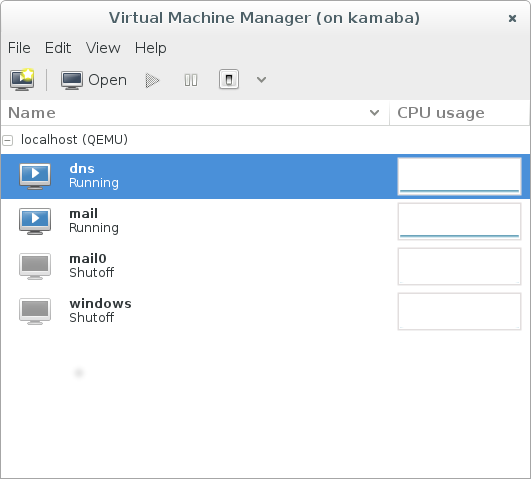
\includegraphics{image201404/virt-manager.png}
\caption{virt-manager$B$N?^(B}
\end{figure*}

\subsubsection{$B2>A[(Bbridge$B$N:n@.(B}
$B<!$K!"2>A[(Bbridge$B$r:n@.$7$^$9!#$3$l$O!"%=%U%H%&%'%"$G(B802.1d Ethernet$B%V%j%C%8$r<BAu$7$F$$$^$9!#(B
$B<j=g$H$7$F$O!"(B
\begin{enumerate}
\item br0$B$r:n@.(B
\item eth0$B$r=i4|2=!"(Bbr0$B$K@\B3(B
\item VM$B$N2>A[(BNIC$B$KBP1~$9$k%$%s%?!<%U%'%$%9$r(Bbr0$B$K@\B3(B
\end{enumerate}

$B6qBNE*$K$O!"(Bvirt-manager$B$rN)$A>e$2!V(BConnection Details$B!W$G!"!V(BNetworkInterfaces$B!W$N!V(BConfigure network interface$B!W$G!V(BBridge$B!W$rA*Br$7!"2>A[(Bbridge$B$K$9$k%G%P%$%9$rA*Br$7$F(BIP$B%"%I%l%9!J(BIPv4$B!K$r$U$j$^$9!#(B

%$B?^7A$NA^F~(B
\begin{figure*}[!b]
\centering
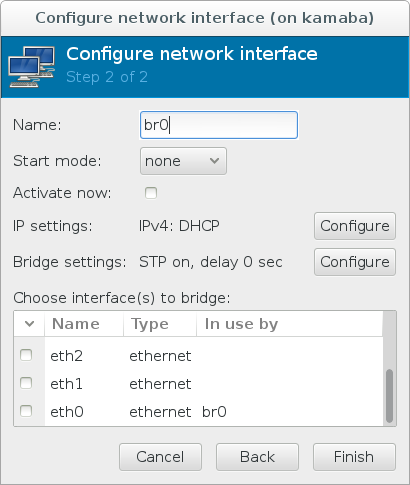
\includegraphics{image201404/bridge2.png}
\caption{bridge$B@_Dj$N>\:Y$N?^(B}
\end{figure*}
\clearpage

$B8e$O!"(BVM$B$r:n@.$9$k$H$-$K%M%C%H%o!<%/$G!V(Bbridge$B!W$rA*Br$9$l$P$$$$$@$1$G$9!#(B
$B%$%a!<%8$H$7$F$O0J2<$N!V?^!W$N$h$&$K$J$j$^$9!#(B

$B$3$3$G(Beth0$B$O!V(Bbridge$B!W$H$7$F30It$K$D$J$,$j$^$9!#$^$?!"%;%-%e%j%F%#$N4X78$+$i(Beth1$B$OJL!V(Bsegment$B!W$K$7!"(Beth0$B$+$iDL?.$r<WCG$7$^$9!#$3$N(Beth1$B$G$O(BSSH$B$J$I$r;HMQ$7!"(Bvirt-manager$B$G3F(BVM$B$r4IM}$7$^$9!#$=$7$F(Beth2$B$O(Beht0$B$HF1$8!V(Bsegment$B!W$K$7$F!"8e=R$N(BSpice$B@lMQ$H$7$^$9!#(B

\begin{figure*}[!h]
\centering
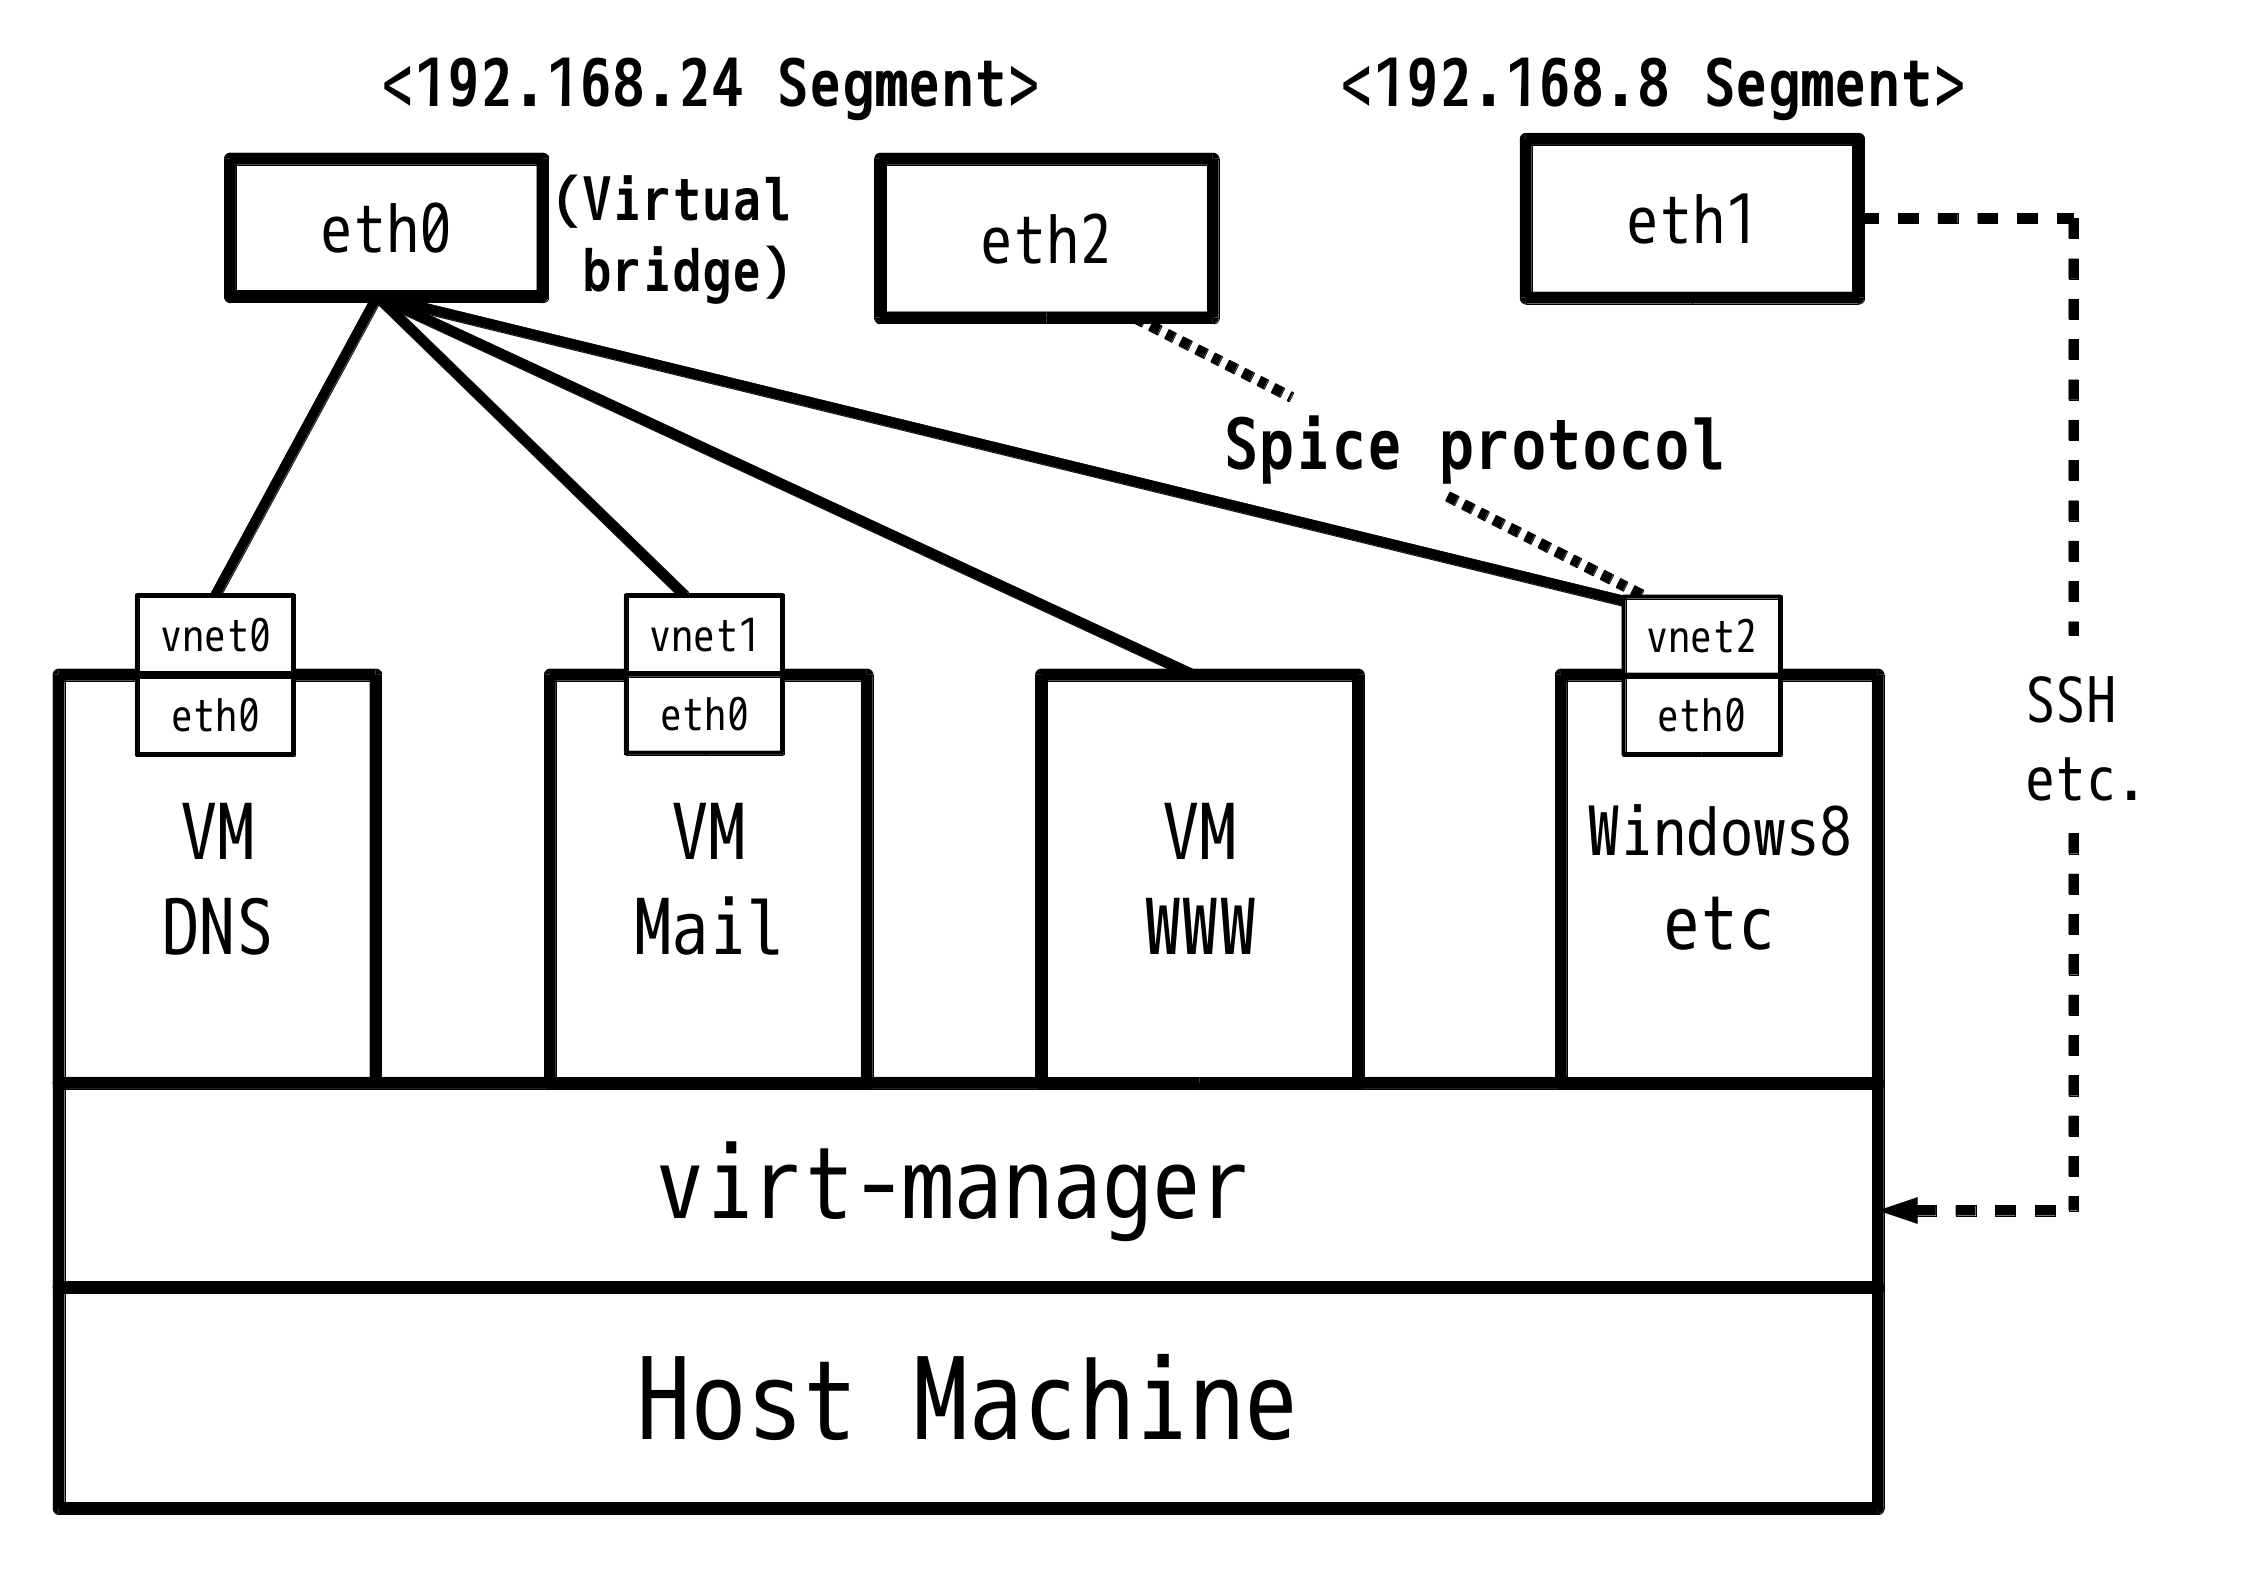
\includegraphics[scale=0.3]{image201404/kvmnetwork3.png}
\caption{$B%M%C%H%o!<%/9=@.$N?^(B}
\end{figure*}

\subsubsection{Virtual Machine$B$N:n@.(B}
$B<!$K!"(Bvirt-manager$B$G(BVM$B$r:n@.$7$^$9!#(Bvirt-manager$B$O(BGUI$B%D!<%k$N%&%#%6!<%I$G!"(BVM$B$N:n@.;~$K$O!"J*M}%^%7%sMQ$N%$%s%9%H!<%k%G%#%9%/!J;THN(BOS$B!K$d(BISO$B%$%a!<%8$r;H$$(BVM$B$r:n@.$7$^$9!#$^$?!"<B%^%7%s$N%j%=!<%9Fb$G$"$l$PMF0W$K(BVM$B$N!V3HD%!W$,$G$-$^$9!#(B
%Hands on$B$K$h$k%$%s%9%H!<%k(B 

\clearpage

\subsection{$B3F<o%$%s%?!<%M%C%H4XO"$N%5!<%P$N:n@.(B}
VM$B$N:n@.$,$G$-$?$i!"3F%5!<%P$r:n@.$7$^$9!#$^$:!"(BDNS$B$N:n@.$K$O(Bbind9$B%Q%C%1!<%8$r%$%s%9%H!<%k$7$^$9!#(B
%$B6qBNE*$K(Bwww.kinsen.gr.jp$B$H$$$&%[%9%HL>$KBP1~$9$k(BIP$B%"%I%l%9$r!J:F5"!K8!:w$9$k>l9g!"$^$:!"(Bjp$B%I%a%$%s$N(BIP$B%"%I%l%9$rLd$$9g$o$;$kI,MW$,$"$j$^$9!#$=$N$?$a$K!"%k!<%H%5!<%P$G(Bjp$B%I%a%$%s$N(BIP$B%"%I%l%9$r8!:w$7!"(Bjp$B%5!<%P$K@\B3$7$^$9!#F1MM$K!"(Bjp$B$KB0$9$k(Bgr$B%I%a%$%s$N(BIP$B%"%I%l%9$r8!:w$7!"$5$i$K$O(Bgr$B%I%a%$%s$KB0$9$k(Bkinsen$B$=$7$F(Bwww$B$H=g<!!"3F(BIP$B%"%I%l%9$r8!:w$7!"3F%5!<%P$K@\B3$7$F$$$-$^$9!#$=$7$F:G=*E*$K!"(Bwww.kinsen.gr.jp$B$N(BIP$B%"%I%l%9$,(B203.141.158.41$B$G$"$k;v$,$o$+$j$^$9!#(B
\begin{commandline}
# apt-get install bind9
# apt-get install bind9utils
\end{commandline}
DNS$B$N@_Dj$G$9$,(BNTT$B$N2s@~$N4X78>e!"#18D$N!V%0%m!<%P%k!W(BIP$B%"%I%l%9$7$+;H$($J$+$C$?$N$G!"J#?t$N%m!<%+%k(BIP$B%"%I%l%9$G3F%5!<%P!J%/%i%$%"%s%H!K$K(BIP$B%"%I%l%9$r?6$j$^$9!#$=$3$G!"(Bacl$B!J(BAccess Control List$B!K$G(BIP$B%"%I%l%9$H%M%C%H%o!<%/$r;XDj$7!"(Bacl$B$K%^%C%A$9$k%/%i%$%"%s%H$H!"$=$NB>$N%/%i%$%"%s%H$4$H$KJL!9%>!<%s$rDs6!$7$^$9!#$3$l$rMxMQ$7!"(B1$BBf$N%5!<%P$GFbItMQ!J(Bacl$B$K%^%C%A$9$k!K$H30ItMQ!J(Bacl$B$K%^%C%A$7$J$$!K$N(BDNS$B$r9=C[$7$^$9!#6qBNE*$K$O!"(B
\begin{enumerate}
\item acl$B$G!"%"%I%l%9%^%C%A%j%9%H$r@_Dj!#(B
\item $B%/%i%$%"%s%H!J3F%5!<%P!K$r(BIP$B$K$h$C$F;XDj$7!"%/%i%$%"%s%HKh$N?6$kIq$$$r:n@.!#(B
\item view$B%9%F!<%H%a%s%H$G!"FbIt%/%i%$%"%s%H!"30It%/%i%$%"%s%H$KJL!9$N(Bzone$B%U%!%$%k$r;2>H$5$;$k!#(B
\end{enumerate}
Mailserver$B$K$O!"(BPostfix$B!J(BMTA Mail Transfer Agent$B!K!"(BDovecot$B!J(BMDA Mail Delivery Agent$B!K$r;H$$$^$9!#(B
\begin{commandline}
# apt-get install postfix
# apt-get install dovecot
\end{commandline}
$B$^$:!"(BPostfix$B$K$D$$$F$O!"(Bsasl$B$NG'>Z5!9=$r;H$C$F%f!<%6$NG'>Z!J(BSMPT-AUTH$B!K$r9T$$!"%f!<%6G'>Z$GMQ$$$k%Q%9%o!<%I!JJ?J8!K$r(BTLS$B$G0E9f2=$7$^$9!#$=$7$F!"%a!<%kAw?.$N$?$a$KG'>Z5!G=$N$D$$$?%5%V%_%C%7%g%s%]!<%H$r;HMQ$9$k$?$a$N@_Dj$r$7$^$9!#(B

devecot$B$O(BIMAP$B!J(BInternet Message Access Protocol$B!K%W%m%H%3%k$r;H$$%a!<%k%5!<%P$N%a!<%k$K%"%/%;%9!"A`:n!"%*%U%i%$%s$H%*%s%i%$%s$NAPJ}$GMxMQ$G$-$^$9!#$^$?!"(BMail$B%5!<%P$N9=@.$K$D$$$F$O!"(B
\begin{enumerate}
\item $B<u?.$7$?%a!<%k$r(BMail$B%G%#%l%/%H%j$G07$&$h$&$K@_Dj(B
\item imapcopy$B$r;H$C$F!"5l%a!<%k%5!<%P$h$j%a!<%k%G!<%?$NE>Aw(B
\item $B%&%#%k%9BP:v$K$O!"(Bclamtk$B$r%$%s%9%H!<%k(B
\end{enumerate}

\subsection{$B%5!<%P$N1?MQ!&4IM}(B}
$B%5!<%P!<$N1?MQ!&4IM}$O!"%j%b!<%HA`:n!"%P%C%/%"%C%W!"%P%C%A=hM}$N<B9T!"%H%i%V%k$NM=KI!&H/8+$N$?$a$N2TF/4F;k$J$I$,I,MW$G$9$,!"8D?M$G1?MQ$9$k<+Bp%5!<%P$J$N$G!"(BVM$B$N%/%m!<%s$H(Bimport$B!"(BSPICE$B$r<h$j>e$2$^$9!#(B

\subsubsection{VM$B$N(Bclone$B!"(Bimport}
$B%P%C%/%"%C%W$O!"(BVM$B$G$"$k3F%5!<%P$N%G%#%9%/%$%a!<%8$r%Y!<%9$K!"(Bclone$B$r:n$j$^$9!#$3$N(Bclone$B!J%G%#%9%/%$%a!<%8!K$O%Y!<%9$H$J$C$?(BVM$B$H$^$C$?$/F1$8!V9=@.!W$G$9$,!"(Bvirt-manager$B$r;H$C$F(BMAC$B%"%I%l%9$NJQ99$,$G$-$^$9!#$^$?!"%$%a!<%8$r(BKVM$B$,Av$C$F$$$kJL$N%^%7%s$K(Bimport$B$G$-$^$9!#$^$?!"3F<o%5!<%P$N9=C[$N:]$O!V%Y!<%9$N(BVM$B!W$r:n@.$7!"%/%m!<%s$r:n$C$F!X%+%?%^%$%:!Y$9$k$J$I$N;H$$J}$,$G$-$^$9!#(B

\subsubsection{SPICE}
$B%j%b!<%HA`:n$K$O(BSPICE$B$r;H$$$^$9!#(BSPICE$B!J(BSimple Protocol for Independent Computing Environment$B!K$O!"2>A[2=4D6->e$K9=C[$7$?%G%9%/%H%C%W4D6-$K%j%b!<%H$+$i@\B3$9$k$H$$$&2>A[%G%9%/%H%C%W4D6-!J(BVDI$B!K$G$9!#FCD'$O!"%*!<%W%s%=!<%9$N2hLLE>Aw%W%m%H%3%k$G!"9b2h<A$J%S%G%*E>Aw$H9b2;<A$JAPJ}8~2;@<E>Aw$,$G$-$k$3$H$G$9!#(B

$B<!$K!"(Bspice$B%/%i%$%"%s%H$r%$%s%9%H!<%k$7!"%?!<%_%J%k$+$i@\B3$7$^$9!#(B
\begin{commandline}
# apt-get install spice-client
\end{commandline}
$BB3$$$F!"(Bqemu-kvm$B$N(BVM$B$K@\B3$7$^$9!#(B
\begin{commandline}
$ spicec -h noren.kinsen.gr.jp -p 590X -w *********
\end{commandline}
$B!V(B-h$B!W$O%[%9%HL>!"!V(B-p$B!W$O%]!<%HHV9f!"!V(B-w$B!W$O%m%0%$%s$9$k$?$a$N%Q%9%o!<%I$G$9!#(B

\subsection{$B$^$H$a(B}
$B$^$H$a$H$7$F!"<+J,$N<+Bp%5!<%P$O$3$N4V!"(B2$BG/$[$I!V(BXen$B!W$G1?MQ$7$F$$$^$7$?!#(BXen$B$O(Bqemu-kvm$B$HF1$8%O%$%Q!<%P%$%6$J$N$G$9$,!"2>A[2=$N%b%G%k$,=`2>A[2=$J$N$G!"%5!<%P$KB?$/$N%j%=!<%9$OI,MW$"$j$^$;$s!J%a!<%k%5!<%P!"(BDNS$B$H$b$I$b(B384MB$B$G1?MQ$7$^$7$?!K!#$?$@!"%j%=!<%9$,==J,$KMQ0U$G$-$k$N$G$"$l$P!"(BOS$B$r(Bdefault$B$G;H$($kE@$d!"(Bvirt-manager$B$J$I$N%D!<%k!"!V9bB.!W!V9b5!G=!W$N(BSPICE$B$,;HMQ$G$-$k$J$I$NMxE@$,(Bqemu-kvm$B$K$O$"$j$^$9!#(B

$B:#8e$NM=Dj$H$7$F$O!"(BWWW$B%5!<%P$G$O!V(BHTML5$B!W$r;H$C$?%5%$%H$N9=C[$d!"(BIPv6$B$X$NBP1~!J$?$@$7!"%Q!<%=%J%k%l%Y%k$G(BGlobal Routing Prefix$B$,(B /48-/64bit$BFb$G$"$k$3$H$,A0Ds!K!"$5$i$J$k!X0[<o!Y$N(BOS$B$N(BVM$B2=$r$7$?$$$H;W$C$F$$$^$9!#(B


\dancersection{Notmuch Mail}{David Bremner}

Originally inspired by the sup mail user agent (MUA), notmuch is a GPL3+
set of tools for for dealing with your mail (stored in Maildirs or
similar) via searching and tagging. On top of the C bindings and a
scriptable command line interface, the project directly supports user
interfaces based on Emacs and VIM as well as integration with Mutt. We
also support python, ruby, and go bindings. Other projects based on
notmuch include curses based frontends written in python and Mercury, a
fork of mutt using notmuch as a the backend, a web interface, and a
virtual maildir filesystem.  In this lightning talk I'll give a tour of
the notmuch "ecosystem", concentrating on the Emacs interface and
command line tool.


\dancersection{$B$b$/$b$/$N2q(B}{}

\dancersection{$B:#8e$NM=Dj(B}{Debian JP}

\subsection{$B4X@>(BDebian$BJY6/2q(B}

$B<!2s!"Bh(B84$B2s4X@>(BDebian$BJY6/2q$O(B5$B7n(B25$BF|(B($BF|(B)$B$KJ!Eg6hL1%;%s%?!<$G3+:E$7$^$9!#(B

\subsection{$BEl5~%(%j%"(BDebian$BJY6/2q(B}
$BBh(B113$B2sEl5~%(%j%"(BDebian$BJY6/2q$O(B5$B7n(B17$BF|(B($BEZ(B)$B$K>l=j$OL$Dj$G$9$,3+:EM=Dj$G$9!#(B

%
% $B:};R$K$9$k$?$a$K!"(B4$B$NG\?t$K$9$kI,MW$,$"$k!#(B
% $B$=$N$?$a$ND4@0(B
%% \dancersection{$B%a%b(B}{}
%% \mbox{}\newpage
%% \mbox{}\newpage
%% \mbox{}\newpage

\printindex
%\cleartooddpage

 \begin{minipage}[b]{0.2\hsize}
  \rotatebox{90}{\fontsize{80}{80} {\gt $B4X@>(B Debian $BJY6/2q(B} }
 \end{minipage}
 \begin{minipage}[b]{0.8\hsize}

 \vspace*{15cm}
 \rule{\hsize}{1mm}
 \vspace{2mm}
 
\includegraphics[width=2cm]{image200502/openlogo-nd.eps}
 \noindent \Large \bfseries{Debian $BJY6/2q;qNA(B}\\ \\
 \noindent \normalfont \debmtgyear{}$BG/(B\debmtgmonth{}$B7n(B\debmtgdate{}$BF|(B \hspace{5mm}  $B=iHGBh(B1$B:~H/9T(B\\
 \noindent \normalfont $B4X@>(B Debian $BJY6/2q(B $B!JJT=8!&0u:~!&H/9T!K(B\\
 \rule{\hsize}{1mm}
 \end{minipage}

\end{document}
